\documentclass{article}
\usepackage[thmmarks, framed]{ntheorem} % ntheorem must come before amsmath, or the cross-reference will not be working
\usepackage[utf8]{inputenc}
\usepackage{graphicx} 
\usepackage{booktabs}
\usepackage[a4paper, portrait, margin=1in]{geometry}
\usepackage{amsmath}
\usepackage{amsfonts}
\usepackage{mathtools}
\usepackage{physics}
\usepackage{xcolor}
\usepackage{caption}
\usepackage{subcaption}
% needed for framed theorems
\usepackage{framed} % or, "mdframed"
\usepackage{bm}
\newframedtheorem{frm-res}{Result}
\theorembodyfont{\upshape}
\title{NST IB Mathematical Methods II}
\date{Lent, 2023}
\author{Yu Lu}
\begin{document}
\maketitle
\tableofcontents

\section{Sturm-Liouville Theory}
\subsection{The operator}
A Sturm-Liouville operator
\[
\boxed{
    \mathcal{\MakeUppercase{L}} 
    = -\frac{\mathrm{d}}{\mathrm{d}x} \left( \rho (x) \frac{\mathrm{d}}{\mathrm{d}x}   \right) + \sigma(x), \qquad \rho(x) >0, \, \sigma(x) \in \mathbb{\MakeUppercase{R}} 
}
\]
can be shown to be self-adjoint under appropriate boundary conditions
\[
    \rho \left( vu^{*\prime} - u^* v^\prime \right)\big\rvert_\alpha ^\beta =0,
\]
meaning \( \braket{u}{\mathcal{\MakeUppercase{L}} v} = \braket{\mathcal{\MakeUppercase{L}} u}{v}\) (equivalently, \( {\mathcal{\MakeUppercase{L}} }^{\dagger} = \mathcal{\MakeUppercase{L}} \) ). 

Such self-adjointness provides many convenient features. Just like Hermitian matrices, for example, in the eigenvalue equation for a self-adjoint operator \(\mathcal{\MakeUppercase{L}} y_n = \lambda_{n} y_{n}, \) the eigenvalues $\lambda_{n} $ are real and \textbf{non-degenerate} eigenfunctions $y_n$ are mutually orthogonal. Moreover, the eigenfunctions commonly form a complete basis, from which we could solve inhomogeneous linear differential equations. 

\subsection{A generalisation to any 2nd order linear ODE}
Despite being seemingly restrictive, the Sturm-Liouville operator could express any second order linear differential operator ($a = -p, b = p^\prime -q$)
\[
    \tilde{\mathcal{\MakeUppercase{L}}}
    = p(x) \frac{\mathrm{d}^{2} }{\mathrm{d}x^{2} } + q(x) \frac{\mathrm{d}}{\mathrm{d}x} + r(x)
    = -\frac{\mathrm{d}}{\mathrm{d}x} \left( a(x) \frac{\mathrm{d}}{\mathrm{d}x} \right) - b(x) \frac{\mathrm{d}}{\mathrm{d}x} +r(x)
\]
could be converted into a Sturm-Liouville form by choosing $w(x)$ such that 
\[
    w \tilde{\mathcal{\MakeUppercase{L}} } = 
    - \frac{\mathrm{d}}{\mathrm{d}x} \left( a w \frac{\mathrm{d}}{\mathrm{d}x} \right) + 
    (a w^\prime  - b w) \frac{\mathrm{d}}{\mathrm{d}x} + r w
\]
has a vanishing coefficient for the first derivative term: 
\[ \boxed{
    w(x) = C \exp\left[ \int^x \frac{b(x^\prime )}{a(x^\prime )}\mathrm{d} x^\prime \right] > 0.}
\] 

This way, a Sturm-Liouville operator
\[
    \mathcal{\MakeUppercase{L}} = w(x) \tilde{\mathcal{\MakeUppercase{L}} }
    = -\frac{\mathrm{d}}{\mathrm{d}x} \left( \rho (x) \frac{\mathrm{d}}{\mathrm{d}x} \right) + \sigma (x), \qquad 
    \rho = a w, \, \sigma  = r w 
\]
could be constructed. From this, an eigenvalue problem $\tilde{\mathcal{\MakeUppercase{L}} } y_n = \lambda y_n$ involving $\tilde{\mathcal{\MakeUppercase{L}} }$ could be converted to a generalised eigenvalue problem $\mathcal{\MakeUppercase{L}} y_n = \lambda w(x) y_n$ of the Sturm-Liouville operator $\mathcal{\MakeUppercase{L}}.$ Alternatively, we could stick with the original operator $\tilde{\mathcal{\MakeUppercase{L}}}$ and introduce the weight in the definition of inner product such that
\[
    \braket*{u}{v}_w = \int_{\alpha }^{\beta } w^* u v \,\mathrm{d}x 
    \implies \left\lVert v\right\rVert ^{2}_m = \int_{\alpha }^{\beta } w^* \left\vert v \right\vert ^{2}  \,\mathrm{d}x, 
\]
and the self-adjoint condition becomes 
\( 
    \braket{u}{\mathcal{\MakeUppercase{L}} v}_w = \braket{\mathcal{\MakeUppercase{L}} u}{v}_w.
\) 
Under this convention, $\tilde{\mathcal{\MakeUppercase{L}} }$ satisfying the original eigenvalue equation is self-adjoint with weight $w(x)$ while $\mathcal{\MakeUppercase{L}} $ satisfying the generalised eigenvalue equation is self-adjoint with weight 1. 

\subsection{Solving differential equations}
The eigenfunctions $y_n(x)$ of $\mathcal{\MakeUppercase{L}} $ can often assumed to be orthogonal even in the case of degeneracy
\[
    \mathcal{\MakeUppercase{L}} y_n = \lambda_n w(x) y_n, \quad 
    \braket{y_n}{y_m} = \delta_{nm}. 
\]
For a orthogonal set of eigenfunctions $\{y_n\}$, the completeness condition can be expressed as
\[
    \sum_{n=1}^{\infty} y_n(x) y_n(x^\prime )^{*} = \frac{1}{w(x)} \delta(x - x^\prime). 
\]

Unlike the method of undetermined coefficient, we can always guarentee that our solution to the inhomogeneous equation satisfy the homogeneous boundary conditions if we construct $\{y_n\}$ to meet the boundary conditions. After finding a set of orthogonal eigenfunctions satisfying whatever boundary conditions posed such that
\[
    \mathcal{\MakeUppercase{L}} y_n(x) = \lambda_n w(x) y_n,
\]
the eigenfunction expansion of the solution
\[
    y(x) = \sum_{n=1}^{\infty} a_n y_n(x)
\]
to the equation 
\[
    \mathcal{\MakeUppercase{L}} y(x) = f(x)
\]
can be found by expressing both sides in $\{y_n\},$ multiplying through by $y_m^*$ and invoking the orthogonality (this is slightly different from expanding $f(x)$ in the eigenfunction, which is off by a weight function). This gives
\[
    y(x) = \sum_{k=1}^{\infty} y_k(x) \frac{\braket{y_k}{f}_{w=1}}{\lambda_k},
\]
which is identical to the Green's function method with 
\[
    G(x, x^\prime ) = \sum_{k=1}^{\infty} \frac{1}{\lambda_k} y_k(x) y_k^*(x^\prime ). 
\]

The expansion of any function in the eigenfunction basis is 
\[
    f(x) = \sum_{n=1}^{\infty} y_n(x) \braket{y_n}{f}_w
\]
and this expansion is optical even in the truncated case, giving Bessel's inequality
\[
    \braket{f(x)}_w \geq \sum_{n=1}^{\infty} \left\vert a_n \right\vert ^{2}.
\]

\section{Calculus of variation}
To extremise a functional $F[y] = \int f(x, y, y^\prime )\mathrm{d} x,$ we can set the functional derivative under $y \to  y + \delta y$
\[
    \delta F = \int \delta y \frac{\partial f}{\partial y} + \delta y^\prime \frac{\partial f}{\partial y^\prime } \mathrm{d} x
\]
to zero and use IBP to yield the Euler-Lagrange equation
\[
    \boxed{
    \frac{\partial f}{\partial y} - \frac{\mathrm{d}}{\mathrm{d}x} \left( \frac{\partial f}{\partial y^\prime } \right) = 0, }
\]
with first integrals
\[
    \boxed{
    \frac{\partial f}{\partial x} = 0 \implies 
    f - \sum_{i=1}^{N}  y^\prime \frac{\partial f}{\partial y^\prime } = \text{const},}
\]
\[
    \boxed{
    \frac{\partial f}{\partial y} = 0 \implies 
    \frac{\partial f}{\partial y^\prime } = \text{const}. }
\]
Note that there is only one energy integral. 

Extremising $F[y]$ under the constraint that $G[y] = 0$ is the same as extremising without constraint
\[
    F[y] - \lambda  G[y],
\]
where $\lambda $ is an undetermined constant. 

It is often useful to extremise the functional ($\mathcal{\MakeUppercase{L}} $ is an Sturm-Liouville operator with weight $w(x)$)
\[
    \Lambda[y] = \frac{F[y]}{G[y]} = \frac{\braket{y}{\mathcal{\MakeUppercase{L}}  y}_{w=1}}{\braket{y}_w},
\]
which is achieved when 
\[
    \boxed{
    \mathcal{\MakeUppercase{L}} y = \Lambda w y, }
\]
in other words the extremal values of $\Lambda$ are the eigenvalues of $\mathcal{\MakeUppercase{L}}, $ which can be shown either by doing a constrained optimisation problem with the Euler-Lagrange equation or by extremising the functional from first principle. Note that the minimum value of $\Lambda[y]$ is still larger than the ground state eigenvalue, so this can be used to find the ground state energy (the Rayleigh-Ritz approximation method). 

Fermat's principle states that the functional 
\[
    \int \mu(x) \mathrm{d} x
\]
is extremised for light. 
\section{Laplace's and Poisson's equation}
Many physical systems, including incompressible irrotational fluids, heat conduction, and electrostatics, can be described by Poisson's equation 
\begin{equation}
    \nabla^{2} \Phi(\mathbf{r}) = \rho(\mathbf{r}), 
    \label{eq:Poisson}
\end{equation}
where $\Phi(\mathbf{r})$ is defined in some region $V$ with \textbf{Dirichlet} boundary conditions $\Phi(\mathbf{r} ) = \Psi(\mathbf{r})$ or \textbf{Neumann} boundary conditions $\nabla \Phi \cdot \hat{n} = \Psi(\mathbf{r} )$ on $\partial V.$ Sometimes $\Phi$ is itself an observable, like temperature, while sometimes it is only $\nabla \Phi$ that is physical, like in electrostatics. The distinction sometimes brings about a difference in boundary conditions. We are sometimes (like in heat conduction) also interested in the flux $\mathbf{F} = \kappa \nabla \Phi,$ where $\kappa$ is (piecewise) constant. 

\subsection{Laplace's equation}
When $\rho(\mathbf{r}) = 0$ in Eq.\eqref{eq:Poisson}, it simplifies into Laplace's equation 
\[
    \nabla^{2} \Phi(\mathbf{r} ) = 0,
\]
where $\Phi(\mathbf{r})$ satisfies the same types of boundary conditions as described above. We could express $\Phi (\mathbf{r} )$ as a superposition of separable solutions in cartesian coordinates, planar polar, or spherical polar coordinates. 

\subsubsection{Cartesian coordinates}
Separation into cartesian coordinates gives $\Phi(x,y,z) = X(x)Y(y)Z(z)$ and the Laplace's equation reads 
\[
    \frac{X^{\prime\prime} (x)}{X} + \frac{Y^{\prime\prime} (y)}{Y} + \frac{Z^{\prime\prime} (z)}{Z} = 0, 
\] 
\[
    \implies \frac{\mathrm{d}^{2} X}{\mathrm{d}x} = - k_x ^{2}  X, \quad 
    \frac{\mathrm{d}^{2} Y}{\mathrm{d}y} = -k_y ^{2} Y, \quad 
    \frac{\mathrm{d}^{2} Z}{\mathrm{d}z} = (k_x ^{2} + k_y ^{2} ) Z. 
\]
Therefore, one part of the solution must be qualitatively different from the other two. The most general solution is 
\[
    X = A \cos(k_x x + B) \quad 
    Y = C \cos(k_y y + D), \quad
    Z = E \exp(\sqrt{k_x ^{2}  + k_y ^{2} }z ) + F \exp(-\sqrt{k_x ^{2}  + k_y ^{2} }z ),
\]
but the boundary conditions often immensely simplifies the expression. For example, $k_x$ and $k_y$ may be quantised to integer multiplies of some quantities and $B=D=0$ if oscillatory boundary conditions are given in $X$ and $Y.$ Furthermore, the exponential growth solution in $Z$ are often killed due to regularity constraint at infinity.

\subsubsection{Planar polar coordinates}
In planar polar coordinates, the solution can be separated as $\Phi(r,\phi) = P(\phi) R(r)$ and the Laplace's equation reads 
\[
    \nabla ^{2} \Phi  = \frac{1}{r}\frac{\partial }{\partial r} \left( r \frac{\partial \Phi }{\partial r} \right) 
    + \frac{1}{r^{2} } \frac{\partial ^{2} \Phi }{\partial \phi ^{2} } = 0,
\]
giving the separated ODE as
\[
    \frac{\mathrm{d}^{2} P}{\mathrm{d}\phi } + n^{2} P = 0, \quad 
    r^{2} \frac{\mathrm{d}^{2} R}{\mathrm{d}r^{2} } + r \frac{\mathrm{d}R}{\mathrm{d}r} - n^{2} R = 0,
\]
where $n = 0, 1, 2, \ldots $ from the physical requirement on periodicity of $P$ or $P^\prime$: if $\Phi$ is physically meaningful, then we require $P(\phi + 2\pi ) = P(\phi)$ and if only $\nabla \Phi$ is physical, only $P^\prime$ needs to be periodic. The ODE on $P$ gives oscillatory solution while that on $R$ is of Euler's type and gives a power function solution $R = r^{\pm n}$ or $R = \ln{r}$. Thus, the general solution is 
\[
    \boxed{
    \Phi(r,\phi) = A_0 + B_0 \phi + C_0 \ln{r} + 
    \sum_{\substack{n=-\infty \\ n \neq 0}}^{\infty } r^n (A_n \cos(n \phi ) + B_n \sin(n \phi )).} 
\]
The $B_0 \phi$ term is only present when the physical quantity is $\nabla \Phi.$ Regularity condition at $r=0$ kills $\ln{r}$ and all the $r^{-n}$ while regularity at infinity kills all the $r^{-n}$ dependence (and $\ln{r}$ if it is posted on $\Phi$ itself). Specifying one more boundary condition then gives $A_n$ and $B_n$ in terms of Fourier coefficients. 

The only solution to the Laplace's equation in all space is a constant function, which is consistent with Liouville's theorem in complex analysis (though this is true in 3D as well). Therefore, we usually study the behaviour parts of the space (e.g. a circular disc). Alternatively, we could allow $\hat{n}\cdot \nabla \Phi$ to have a jump discontinuity across some boundaries and split the solution into two piecewise parts. This may correspond to a point source or a discontinuity in the conductivity $\kappa $ (conserving flux $\mathbf{F} $). 

\subsubsection{Spherical polar coordinates}
Laplace's equation in axisymmetric spherical polar coordinates (no $\phi$ dependence) is 
\[
    \nabla ^{2} \Phi = \frac{1}{r^{2} } \frac{\partial }{\partial r} \left(r ^{2} \frac{\partial \Phi }{\partial r} \right) + \frac{1}{r^{2} \sin{\theta }}\frac{\partial }{\partial \theta } \left( \sin{\theta} \frac{\partial \Phi }{\partial \theta } \right) = 0,
\]
where $\Phi(r, \theta) = \Theta(u) R(r)$ and $u = \cos{\theta }.$ The equation can then be separated as
\[
    \frac{\mathrm{d}}{\mathrm{d}u} \left[ (1-u^{2}) \frac{\mathrm{d}\Theta }{\mathrm{d}u} \right] + l(l+1) T = 0, \quad 
    r^{2} \frac{\mathrm{d}^{2} R}{\mathrm{d}r} + 2 r \frac{\mathrm{d}R}{\mathrm{d}r} - l(l+1)r = 0.
\]
The ODE on $\Theta$ is of the Legendre type and is only regular at $u = \pm 1$ when $l = 0, 1, \ldots $ The second ODE is of Euler's type and admits power function solutions $R = r^{l}, r^{-l-1}.$ Thus, the general solution is
\[
    \boxed{ 
        \Phi(r,\theta ) = \sum_{l=0}^{\infty} \left( A_l r^l + B_l r^{-l-1}\right) P_l(\cos{\theta}),
    }
\]
where $P_l(x)$ is the Legendre polynomial with normalisation $P_l(1) = 1.$

(*) When the system is not axisymmetric, the Laplace's equation becomes 
\[
    \nabla ^{2} \Phi = \frac{1}{r^{2} } \frac{\partial }{\partial r} \left(r ^{2} \frac{\partial \Phi }{\partial r} \right) + \frac{1}{r^{2} \sin{\theta }}\frac{\partial }{\partial \theta } \left( \sin{\theta} \frac{\partial \Phi }{\partial \theta } \right) + \frac{1}{r^{2} \sin{\theta }} \frac{\partial^{2}  \Phi }{\partial \phi ^{2} } = 0. 
\]
It needs to be separated into $\Phi(r,\theta,\phi) = R(r) \Theta(\theta ) P(\phi )$ with two separation constants, as shown below:
\[
    \begin{dcases}
       \frac{\sin^{2}{\theta }}{R} \frac{\mathrm{d}}{\mathrm{d}r} \left( r^{2} \frac{\mathrm{d}R}{\mathrm{d}r} \right) + \frac{\sin{\theta }}{\Theta}\frac{\mathrm{d}}{\mathrm{d}\theta } \left( \sin{\theta } \frac{\mathrm{d}\Theta }{\mathrm{d}\theta } \right)  = -\frac{1}{P}\frac{\mathrm{d}^{2} P}{\mathrm{d}\phi ^{2} } &= \lambda_1,   \\
       \frac{1}{R}\frac{\mathrm{d}}{\mathrm{d}r} \left(r^{2} \frac{\mathrm{d}R}{\mathrm{d}r} \right) = -\frac{1}{\Theta \sin{\theta }}\frac{\mathrm{d}}{\mathrm{d}\theta } \left( \sin{\theta } \frac{\mathrm{d}\Theta }{\mathrm{d}\theta } \right) + \frac{\lambda_1}{\sin^{2}{\theta }} &= \lambda_2.    
    \end{dcases}
\]
\subsection{Uniqueness of solutions to Poisson's equation} 
The uniqueness theorem states that if $\nabla^{2} \Phi = \rho(\mathbf{r})$ in $V$ and Dirichlet or Neumann boundary conditions are satisfied on $\partial V,$ then the solution must be unique, or unique up to a constant for Neumann conditions. This can be proved by showing that $\Psi = \Phi_2 - \Phi_1 $ satisfies 
\[
\int_{V}^{} \left\vert \nabla \Psi  \right\vert ^{2}  \,\mathrm{d}V  = 
    \oint_{\partial V} \Psi \nabla \Psi \cdot \mathrm{d}\mathbf{S} = 0
\]
using the vector identity $\boxed{\nabla\cdot(\Psi \nabla \Psi) = \left\vert \nabla \Psi  \right\vert ^{2} + \Psi \nabla ^{2} \Psi}. $ 

This allows us to use the method of image to convert Poisson's equation in a confined space to a Poisson's equation over all space. 
\subsection{Green's function to a point source}
Green's function to the Poisson's equation in $V$ bounded by $S$ is 
\[
    \boxed{
        \nabla_r ^{2} G(\mathbf{r}, \mathbf{r^\prime }) = \delta^{(3)}(\mathbf{r}-\mathbf{r^\prime })
    }
\]
satisfying homogeneous $\boxed{G = 0 \text{ on } S}$ for a Dirichlet problem or $\boxed{\nabla \cdot G = 1/A \text{ on } S}$ for a Neumann problem, where $A$ is surface area of $S$ and $\mathbf{r^\prime }$ can be any point inside $V.$ It is not hard to verify that $G(\mathbf{r}, \mathbf{r^\prime } )$ is symmetric under $\mathbf{r}  \Leftrightarrow \mathbf{r^\prime }.$ The condition on Neumann problem comes from conserving the flux 
\[
    \oint_S \nabla G \cdot \mathrm{d}\mathbf{S} = \int_{V}^{} \nabla ^{2} G \,\mathrm{d}V = \int_{V}^{} \delta^{(3)}(\mathbf{r}-\mathbf{r^\prime }) \,\mathrm{d}V=1. 
\]
\subsubsection{3D fundamental solution}
A fundamental solution $G(\mathbf{r}, \mathbf{r^\prime })$ is the Green's function satisfying the boundary conditions in the whole space. Just as what we did in finding the Green's function of an ODE, $G$ can be obtained by solving the Laplace's equation but allowing for discontinuity with determined strength at the origin. 

Since the proposed PDE is radially symmetric, we would expect $G$ to only have radial dependence, giving
\[
    \nabla^{2} G = \frac{1}{r^{2} }\frac{\partial }{\partial r} \left( r^{2} \frac{\partial G}{\partial r} \right) = 0 \quad \implies  G = \frac{C}{r}+A \quad (r \neq 0),
\]
where $A, C$ are arbitrary constants. The constant offset $A$ must be $0$ for a Dirichlet problem but can be left undetermined for a Neumann problem. The strength $C$ can be determined by the flux out from the origin:
\[
    \int_{r<\epsilon} \nabla^{2} G \mathrm{d} V = \oint_{r = \epsilon } \frac{\partial G}{\partial r} \mathrm{d} S = 1, 
\]
giving (shifting the origin)
\[
    \boxed{
        G = -\frac{1}{4\pi \left\vert \mathbf{r} - \mathbf{r^\prime }  \right\vert }. 
    }
\]
\subsubsection{2D fundamental solution}
Similarly, the fundamental solution to the 2D Poisson's equation 
\[
    \nabla_r ^{2} G(\mathbf{r}, \mathbf{r^\prime } ) = \delta^{(2)} (\mathbf{r} - \mathbf{r^\prime } )
\]
is
\[
    \boxed{ 
        G(\mathbf{r} , \mathbf{r^\prime } ) = \frac{1}{2\pi } \ln{\left\vert \mathbf{r} - \mathbf{r^\prime }  \right\vert } + \mathrm{const}. 
    }
\]
Note that in two dimensions we can no longer require $G \to 0$ at infinity, so the Dirichlet boundary conditions are usually specified in other ways. 
\subsubsection{The method of image for complicated geometry}
We can seek Green's function over a infinite domain using the fundamental solution. However, we often want to find Green's functions in some more complicated domains, like a half-plane or a circle. This calls for the method of image which relies on uniqueness of solution to Poisson's equation. If we can cleverly introduce point sources \textbf{outside} the domain $V$ such that the fundamental solution over the whole space also \textit{happens} to satisfy the homogeneous boundary condition on the finite domain $V,$ we can claim to find the \textbf{unique} solution. 
\begin{figure}[ht]
    \centering
    \begin{subfigure}{.5\textwidth}
      \centering
      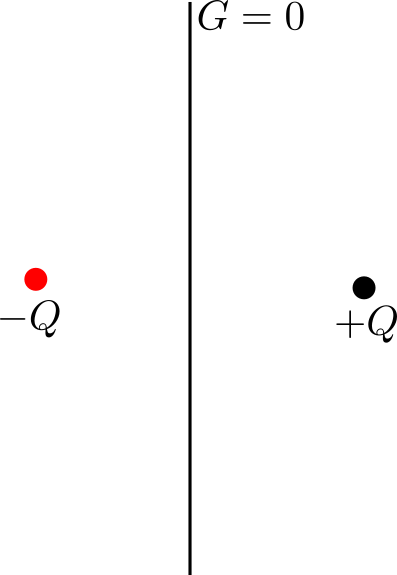
\includegraphics[width=.4\linewidth]{figs/chap3_image_point_dirichlet.png}
      \caption{Dirichlet boundary condition}
    \end{subfigure}%
    \begin{subfigure}{.5\textwidth}
      \centering
      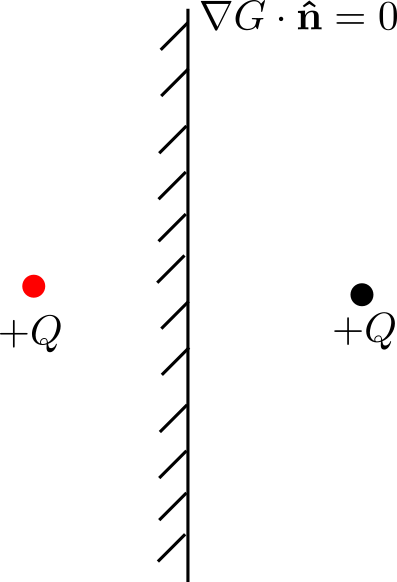
\includegraphics[width=.4\linewidth]{figs/chap3_image_point_neumann.png}
      \caption{Neumann boundary condition}
    \end{subfigure}
    \caption{Image charges (red) for an infinite plane boundary conditions.}
    \label{fig:chap3-image-plane}
    \end{figure}

For example, for a infinite plane/line boundary, we could simply reflect the source, as shown in Fig.\ref{fig:chap3-image-plane} to give the Green's function as a superposition of fundamental solutions:
\[
    G = -\frac{1}{4\pi }\left( \frac{1}{\left\vert \mathbf{r} - \mathbf{r_0}  \right\vert } \pm \frac{1}{\left\vert \mathbf{r} - \mathbf{r_1}  \right\vert }\right),
\]
where $\mathbf{r_1}$ is the position of the image charge. With Dirichlet boundary conditions, an image source of opposite sign is introduced and we essentially have a dipole field with all flux through the wall (none to infinity). With Neumann boundary conditions, on the other hand, all the flux spreads out to infinity.

For a spherical or circular boundary with Dirichlet boundary condition, we could put an image charge at the inverse point $\mathbf{x_1} = (a^{2} / \left\vert \mathbf{r_0}  \right\vert ) \mathbf{r_0} $ (so that $a$ is the geometric mean of $r_0$ and $r_1$). For a 2D circle, the strength of the image charge is just $q = -Q$ while for a 3D sphere the image charge must have a weaker strength $q = -a/r_0.$
\begin{figure}[ht]
    \centering
    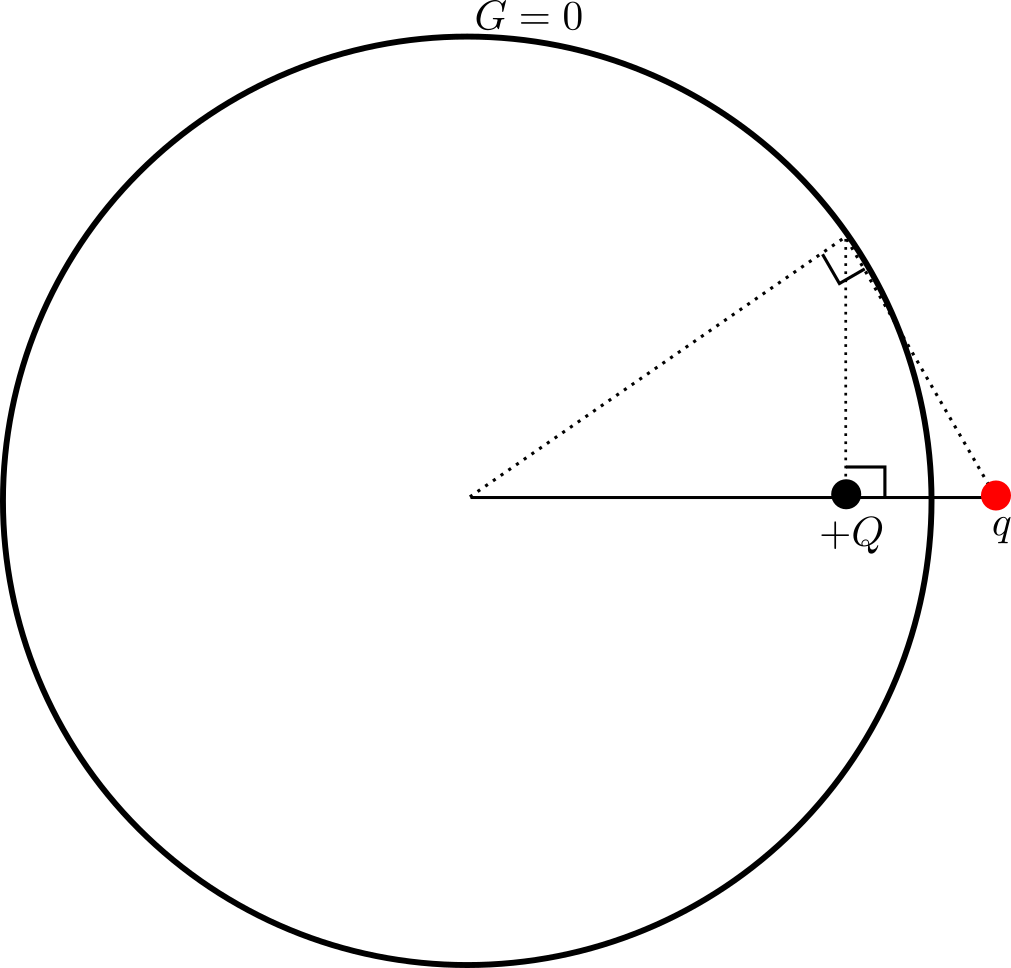
\includegraphics[width=0.4\textwidth]{figs/chap3_inverse_point_dirichlet.png}
    \caption{Inverse point for a spherical or circular Dirichlet boundary.}
    \label{fig:chap3-inverse}
\end{figure}

If the boundary is in more complicated geometry, some numerical methods are probably needed to find the Green's function. However, an inhomogeneous forcing or an inhomogeneous boundary condition with a simple geometry could be resolved by the following integral solution. 
\subsection{Integral solution to Poisson's equation}
With the Green's function in hand, we could solve the inhomogeneous Poisson's equation $\nabla ^{2} \Phi = \rho(\mathbf{r} )$ with inhomogeneous boundary condition $\Phi = f(\mathbf{r})$ on $S$ or $\nabla \Phi \cdot \mathbf{\hat{n} } = f(\mathbf{r})$ on $S.$ From the same vector calculus identity we used in proving uniqueness of Poisson's equation, we could prove Green's second identity ($\Psi = G$ )
\[
    \boxed{ 
        \int_V = (\Phi \nabla^{2} \Psi  - \Psi \nabla ^{2} \Phi ) \mathrm{d} V = 
        \oint_S \left( \Phi \frac{\partial \Psi }{\partial n} - \Psi \frac{\partial \Phi }{\partial n} \right). 
    }
\]
For a Dirichlet boundary condition, this simplifies to 
\[
    \boxed{
        \Phi (\mathbf{r^\prime } ) = \int_V \rho(\mathbf{r} ) G(\mathbf{r}, \mathbf{r^\prime } ) \mathrm{d} V + \oint f(\mathbf{r} ) \nabla G \cdot \mathrm{d} \mathbf{S},  
    }
\]
where the first term comes from superposition of different sources and the second term comes from inhomogeneous boundary conditions. Similarly, the solution from Neumann boundary condition is
\[
    \boxed{ 
        \Phi (\mathbf{r^\prime } ) = \int_V \rho(\mathbf{r} ) G(\mathbf{r}, \mathbf{r^\prime } ) \mathrm{d} V - \oint f(\mathbf{r} ) G(\mathbf{r}, \mathbf{r^\prime } ) \mathrm{d}S + C.
    }
\]

\section{Cartesian Tensors}

\[
    L_{ij} = \mathbf{e_i^\prime } \cdot \mathbf{e_j}, \quad L L^{\top}  = I
\]
and $v_i$ is a tensor of order one if
\[
    v_i^\prime  = L_{ij} v_j; 
\]
it is a axial-vector if 
\[
    v_i^\prime  = \mathrm{det}(L)  L_{ij} v_j; 
\]

An antisymmetric second-order tensor can be associated with an axial vector as
\[
    A_{ij} = \epsilon_{ijk} \omega_k, \quad 
    \omega_k = \frac{1}{2} \epsilon_{klm} A_{lm}. 
\]
Any symmetric second-order tensor $S$ can be decomposed into an isotropic tensor and a traceless tensor $\tilde{S}$
\[
    S = \tilde{S} + \frac{1}{3}\mathrm{Tr}(S)\mathbb{I}.
\]

Any symmetric tensor can be diagonalised (it has real eigenvalues and eigenvectors) by a change of basis into the eigenbasis 
\[
    S^\prime = L S L^{\top}. 
\]

The moment of inertia tensor is 
\[
    I_{ij} = \int \rho(\mathbf{x} ) (x_k x_k \delta_{ij} - x_i x_j) \mathrm{d} V.  
\]

All scalars are isotropic; all first order isotropic tensors are zero; the most general second order isotropic tensor is $\lambda \delta_{ij}$; the most general third order isotropic tensor is $\lambda  \epsilon_{ijk}.$ It can be argued that integrals over the symmetric volume 
\[
    X_i = \int_{V} x_i \rho(r) \mathrm{d} V, \quad 
    K_{ij} = \int_{V} x_i x_j \rho(r) \mathrm{d} V
\]
are both isotropic. The undetermined coefficient in $K_{ij}$ can be found by calculating a trace, which is just one integral. 
\end{document} 